%% Copernicus Publications Manuscript Preparation Template for LaTeX Submissions
%% ---------------------------------
%% This template should be used for copernicus.cls
%% The class file and some style files are bundled in the Copernicus Latex Package, which can be downloaded from the different journal webpages.
%% For further assistance please contact Copernicus Publications at: production@copernicus.org
%% https://publications.copernicus.org/for_authors/manuscript_preparation.html

%% copernicus_rticles_template (flag for rticles template detection - do not remove!)

%% Please use the following documentclass and journal abbreviations for discussion papers and final revised papers.

%% 2-column papers and discussion papers
\documentclass[, manuscript]{copernicus}



%% Journal abbreviations (please use the same for discussion papers and final revised papers)


% Advances in Geosciences (adgeo)
% Advances in Radio Science (ars)
% Advances in Science and Research (asr)
% Advances in Statistical Climatology, Meteorology and Oceanography (ascmo)
% Annales Geophysicae (angeo)
% Archives Animal Breeding (aab)
% ASTRA Proceedings (ap)
% Atmospheric Chemistry and Physics (acp)
% Atmospheric Measurement Techniques (amt)
% Biogeosciences (bg)
% Climate of the Past (cp)
% DEUQUA Special Publications (deuquasp)
% Drinking Water Engineering and Science (dwes)
% Earth Surface Dynamics (esurf)
% Earth System Dynamics (esd)
% Earth System Science Data (essd)
% E&G Quaternary Science Journal (egqsj)
% Fossil Record (fr)
% Geochronology (gchron)
% Geographica Helvetica (gh)
% Geoscience Communication (gc)
% Geoscientific Instrumentation, Methods and Data Systems (gi)
% Geoscientific Model Development (gmd)
% History of Geo- and Space Sciences (hgss)
% Hydrology and Earth System Sciences (hess)
% Journal of Micropalaeontology (jm)
% Journal of Sensors and Sensor Systems (jsss)
% Mechanical Sciences (ms)
% Natural Hazards and Earth System Sciences (nhess)
% Nonlinear Processes in Geophysics (npg)
% Ocean Science (os)
% Primate Biology (pb)
% Proceedings of the International Association of Hydrological Sciences (piahs)
% Scientific Drilling (sd)
% SOIL (soil)
% Solid Earth (se)
% The Cryosphere (tc)
% Web Ecology (we)
% Wind Energy Science (wes)


%% \usepackage commands included in the copernicus.cls:
%\usepackage[german, english]{babel}
%\usepackage{tabularx}
%\usepackage{cancel}
%\usepackage{multirow}
%\usepackage{supertabular}
%\usepackage{algorithmic}
%\usepackage{algorithm}
%\usepackage{amsthm}
%\usepackage{float}
%\usepackage{subfig}
%\usepackage{rotating}

% The "Technical instructions for LaTex" by Copernicus require _not_ to insert any additional packages.
%


\begin{document}

\title{Fire danger: the skill provided by the ECMWF Integrated Forecasting
System}


\Author[1]{Francesca}{Di Giuseppe}
\Author[1]{Claudia}{Vitolo}
\Author[1]{Blazej}{Krzeminski}
\Author[2]{Jesus}{San-Miguel}
\Author[1]{Florian}{Pappenberger}


\affil[1]{European Centre for Medium-range Weather Forecasts, Reading, United
Kingdom}
\affil[2]{European Commission, Joint Research Centre, Ispra, Italy}

%% The [] brackets identify the author with the corresponding affiliation. 1, 2, 3, etc. should be inserted.



\runningtitle{Fire danger forecasting}

\runningauthor{Di Giuseppe et al.}


\correspondence{Francesca\ Di Giuseppe\ (F.DiGiuseppe@ecmwf.int)}



\received{}
\pubdiscuss{} %% only important for two-stage journals
\revised{}
\accepted{}
\published{}

%% These dates will be inserted by Copernicus Publications during the typesetting process.


\firstpage{1}

\maketitle


\begin{abstract}
In the framework of the EU Copernicus program the European Centre for
Medium-range Weather Forecast (ECMWF) on behalf of the Joint Research
Centre (JRC) is forecasting daily fire weather indices using its medium
range ensemble prediction system. The use of weather forecast in place
of local observations can extend early warnings up to 1-2 weeks allowing
for greater proactive coordination of resource-sharing and mobilization
within and across countries. In addition, the use of an ensemble system
allows to perform a probabilistic assessment of the forecast
uncertainties which can boost confidence in the decision process during
emergency situations. Using one year of pre-operational service in 2017
here we assess the capability of the system globally and analyze in
detail three major events in Chile, Portugal and California. We also
present examples on how fire forecast products could be tailored to
provide uncertainties of fire weather conditions and information in a
probabilistic fashion.
\end{abstract}




\introduction

The prediction of fire danger conditions allows forestry agencies to
implement fire prevention, detection, and pre-suppression action plans
before fire damages. However, in many countries fire danger rating
relies on observed weather data which only allows for daily
environmental monitoring of fire conditions \citep{taylor:06}. Even when
this estimation is enhanced with the combined use of satellite data,
such as hot spots for early fire detection, and land cover and fuel
conditions it normally only provides 4- to 6-hour warnings. By using
forecast conditions from advanced numerical weather models, early
warning could be extended up to 1-2 weeks allowing for greater
coordination of resource-sharing and mobilization within and between
countries.

Due to the improved skills of weather forecasting, the use of numerical
weather prediction offers a real opportunity to enhance early warning
capabilities \citep{roads:05,molders:08,molders:10}. In recent years
institutions such as Natural Resources Canada (NRC) and the US National
Oceanic and Atmospheric Administration (NOAA) have implemented regional
fire danger forecasting systems based on their operational weather
forecasts \citep{bedia:18}. The Global Fire Early Warning System is also
an international initiative, promoted by the Canadian Parternship for
Wildland Fire Science and the United Nation Office for Disaster Risk
Reduction, to provide fire danger forecast up to 10 days ahead using the
Canadian operational weather forecasting system
(\url{http://canadawildfire.ualberta.ca/gfews}). Parallel initiatives
are promoted by the European Commission under the umbrella of the
Copernicus Emergency Management Service (CEMS), namely the European Fire
Forecast Information System (EFFIS,
\url{http://effis.jrc.ec.europa.eu/}) and its global counterpart the
Global wildfire Information System (GWIS,
\url{http://gwis.jrc.ec.europa.eu/}). Both systems rely on the Canadian
Fire Weather Index (FWI) \citep{vanwagner:74,vanwagner:85} to rate fire
danger and on numerical weather predictions to provide forecasted fire
danger information at the European and global levels
\citep{sanmiguel:02}.

Systems such as the FWI detect dangerous weather conditions conducive of
uncontrollable fires rather than modelling the probability of ignition
and fire behaviours. The FWI (developed in Canada) is specifically
calibrated to describe the fire behaviour in a jack pine stand
(\emph{Pinus banksiana}) typical of the Canadian forests. However, its
simplicity of implementation has made it a popular choice in many
countries and it has shown to perform reasonably well in ecosystems very
dissimilar to the boreal forest \citep{digiuseppe:16,degroot:07}. The
FWI calculation only relies on weather forcings and no information on
the actual vegetation status is taken into account. When weather
forecasts are used in place of observations, uncertainties can be
introduced. Sources of uncertainty can be: (i) the limited
predictability of atmospheric dynamics which is strongly affected by the
initial state and (ii) the misrepresentation of physical processes. In
the former case, errors are randomly distributed around the true state
\citep{orrell:01}; in the latter, errors produce systematic deviations
from the true state. In both cases, errors in the weather forecast may
be amplified or damped by nonlinear transformations in the fire weather
model \citep{erickson:18}. Thus, for example, a dry bias in the model in
a certain region will lead to the persistent prediction of higher fire
danger values compared to what would be calculated using local
observations.

Handling random errors in weather forecasts is traditionally done
through the use of ensemble prediction systems where several simulations
are performed starting from slightly different initial conditions and
model configurations \citep{molteni:96,buizza:99}. The forecast is then
interpreted as probabilistic rather than deterministic. While it has
been shown that the probabilistic information contained in an ensemble
prediction system might be difficult to interpret for end-users
\citep{pappenberger:13}, ensembles can also boost confidence in the
decision process during emergency situations as a cost-loss analysis can
be associated to the different scenarios \citep{cloke:17}. Moreover,
ensemble predictions can have more information value than the single
deterministic simulation \citep{richardson:00,zhu:02}. Systematic
biases, on the other hand, can be reduced by model improvements. Still
appropriate post-processing (bias correction) of the atmospheric model
\citep{piani:10,digiuseppe:13a,digiuseppe:13b} or post-processing of the
sectoral application outputs \citep{raftery:05} can correct resolved
processes and improve the final forecast skill.

Given the above considerations, in this paper we assess the performance
of the fire danger forecasting system developed for the Copernicus
Emergency Management Service at European Centre for Medium-range Weather
Forecasts (ECMWF) to predict the FWI values and the probability of
detection of fire during one year of operation in 2017. As the Fire
Weather Index is the main index of this system we will concentrate on
this model component.

\subsection{FWI calculation}\subsubsection{General concept}

The Fire Weather Index system is composed of six variables describing
fuel moisture and fire behavior, as influenced by weather
\citep{vanwagner:87}. Three fuel moisture codes provide the moisture
content of dead woody debris of different diameter classes laying on
three fuel beds. The dead fine fuels is described by the Fine Fuel
Moisture Code (FFMC) which has a fast response time to weather
modification (hourly time scales). The surface organic matter of
moderate density, such as the fermentation layer of forest soils
\citep{hood:10} is calculated using the Duff Moisture Code (DMC). DMC
has a slower response to the weather forcing, conventionally set to 12
days. Finally the deep, compact soil organic layers, such as the humus
layer of forest soils \citet{hood:10} is expressed with a Drought Code
(DC). This is the slower evolving component of the FWI codes and has a
lag-time set to 52 days in the original FWI formulation. The FWI system
also provides fire behavior indexes, in terms of rate of fire spread
(Initial Spread Index, ISI), fuel available for combustion (Buildup
Index, BUI), and head fire intensity (Fire Weather Index, FWI). The FWI
component combines the ISI and BUI and can be considered as the most
general indicator of fire danger.

A comprehensive description of the FWI system, the interaction between
the various components and how these are used in fire management can be
found in \citep{vanwagner:87,wotton:09}. In the interest of brevity we
have here only recalled the basic concepts underlying the FWI system and
how different components might be more appropriate to describe fire
danger depending on the local fuel characteristics and the type of
information required. \cite{abatzoglou:18} showed that FWI exhibits
strong correlative relationships to burned area across most non-arid
eco-regions globally, while \citet{bowman:17} highlighted how high FWI
values are often associated to the most extreme fire activities recorded
using Fire Radiative Power observations. As FWI has been shown to
provide a good metric for quantifying fire danger globally, the proposed
analysis of forecast skills will concentrate on this index
\citep{digiuseppe:16,degroot:07}.

\subsubsection{FWI forecast}

For each day indexes of the FWI rating system are calculated
operationally at ECMWF using real-time (RT) forecasts. A full
description of the modeling components can be found in
\citet{digiuseppe:16}. The high resolution (HRES) and the ensemble
prediction systems (ENS) provide weather forecasts which extend up to 10
days in the future. The atmospheric forcings have a temporal resolution
of 3 hours and a spatial resolution of 9km for the high resolution run
and 18 km for the ensemble prediction simulations. While the HRES is a
single (deterministic) model integration, the ENS provides 51
realizations from perturbed initial conditions and different model
physics \citep{buizza:99}. These ENS forecasts are used to assess
uncertainties in the prediction.

A model integration at any nominal time simulates atmospheric conditions
at a different local time, depending on the location. FWI calculations
are usually performed at 12:00 local time because the model was
calibrated using measurements at 12:00 against fire behavior the most
active window (between 14:00-16:00) \citep{vanwagner:87}. Therefore to
produce a snapshot at 12:00 local time, a temporal and spatial collage
of 24 hours time model simulations is performed. Atmospheric fields are
cut into 3-hourly time strips using the closest 3-hour forecast outputs
and then concatenated together so that the final field is representative
of the conditions around the local noon within the 3 hour resolution
available \citep{digiuseppe:16}.

\subsubsection{FWI reference and benchmark}

As many forestry agencies still rely on observed meteorological data to
provide fire danger, a first assessment of the quality of forecasted FWI
will rely on the comparison with observations. Despite several
meteorological observations are available through the Global
Telecommunication System (GTS) SYNOP network, only a subgroup of
stations have at least 30 days of recordings at local noon during 2017
(spatial coverage is given in figure \ref{fig:synop}). Many fire prone
regions, such as Australia, would not be covered by this comparison. In
order to overcome this limitation, a reference dataset of FWI modelled
values is also used. This is constructed using the ERA5 reanalysis
dataset. ERA5 is the latest of ECMWF reanalysis products which was
released at the beginning of 2019. It substitutes the previous
ERA-Interim database \citep{dee:11,vitolo:19} providing a much improved
spatial resolution and an extensive increment of assimilated
observations. Simulations begin in 1979 and are updated in quasi real
time. Fields have a spatial resolution of about 30 km and hourly time
resolution. Outputs from ERA5 undergo the same temporal interpolation
described in the previous section to provide the model with a composite
fire reanalysis product at 12:00 local time. It has to be noted that,
compared to local observations, a reanalysis provides a dynamically
consistent estimate of the climate state at each time step and can, to a
large extent, be considered a good proxy for observed meteorological
conditions. Moreover, by combining different observations, reanalysis
datasets extend well beyond the natural life of single observational
networks and they can provide a wider spatial coverage than using local
observations.

In addition, from ERA5 we derive a climatological benchmark simulation
(called CLIM hereafter), considered as a ``mean year'' for the FWI using
the period 1980-2018. At pixel level, every day the median FWI is
calculated over the period spanning 4 days before/after a given date.
While CLIM has no expected predictive skill for a specific year, it
retains information on the yearly climatological variation of FWI. CLIM
is what could be used in the absence of either a monitoring (based on
observations) or a forecast system (based on weather forecast). It
should therefore score better or equal of the forecast on time ranges
beyond the limits of predictability. CLIM is used in this study as a
benchmark to rank the expected improvements provided by a forecasting
system

\subsection{Observed fire events}

While national inventories of wildfire activities exist in many
countries, they can be heterogeneous and lack the temporal span
desirable for the validation of a fire danger system at the global
scale. Satellite observations can supply a valid alternative especially
as they cover remote areas where in-situ observations are sparse
\citep{flannigan:86,giglio:03,schroeder:08}. Daily maps of fire
radiative power (FRP) \citep{kaufman:03,wooster:05} are available from
ECMWF since 2003 through the Global Fire Assimilation System (GFAS)
\citep{kaiser:2012,digiuseppe:17,digiuseppe:18}. This dataset has been
developed in the framework of the Copernicus Atmosphere Monitoring
Services (CAMS) and uses observations from the MODIS sensors on board of
Terra and Aqua platforms and assumptions on fire evolution to calculate
a continuous record of active fires. The GFAS dataset integrates all
available FRP observations available in a day over a regular \(0.1\deg\)
grid. According to \citet{wooster:05}, this provides an indication of
the cumulative dry mass available for burning which can be then put into
a relationship with fire emissions. In this paper, the FRP products are
only used as an observations of fire events. However, FRP values are
ignored and only used to derive a mask of fire occurrence based on a
minimum detection criteria: \(FRP> 0.5 Wm^{-2}\) \citep{kaiser:2012}. A
``hit'' is recorded if the fire forecast predicts fire danger above the
95\textsuperscript{th} percentile of its historical values (provided by
the ERA5 simulations) when a fire really occurred.

\subsection{Score metrics}

The performance of the the fire forecasting systems to reproduce
observed FWI values is assessed using deterministic and probabilistic
scores. Both the synop database and ERA5 are treated as a proxy for
observations in the evaluation. To asses the quality of the computation
we use traditional deterministic skill scores such as the mean bias (MB)
and the mean absolute error (MAE). For a probabilistic assessment, the
continuous ranked probability score is also employed (CRPS;
\cite{hersbach2000}). These are defined as:

\begin{align}
MB&=\sum_{p=1}^{cases}\left[F_{n=HRES}-O\right]\\
MAE&=\frac{1}{cases}\sum_{p=1}^{cases}\sqrt{\left[(F_{n=HRES}-O)^2]\right]}\\
CRPS=\frac{1}{cases}\sum_{t=1}^{cases}\int_{-\inf}^{+\inf}\left[F_{n}-O)^2\right]dn
\end{align}

where F is the forecast at time step t of N number of forecasts and O is
the observed value. While the MB, MAE and the ACC are applied to a
single forecasts, the high resolution forecast, the CRPS takes into
account the whole distribution of possible values predicted by the
ensemble. It is the continuous extension of the ranked probability
score, where \(F_n\) is the cumulative distribution function of the
predicted ensemble values. Then, the CRPS compares the cumulative
probability distribution of the FWI forecasted by the ensemble forecast
system to the observation. In this sense the CRPS is sensitive to the
mean forecast biases as well as the spread of the ensemble
\citep{hersbach2000}.

While conventional skills score can be employed to assess the quality of
the FWI computation, the verification of the FWI as a fire indicator is
instead extremely challenging. First, as widely explained, FWI is not a
physical measure of fire activity but of its potential danger, if one
were ignited. Therefore high fire danger, while being correctly
forecasted, might not result in active fires if there is no ignition.
From the verification point of view this means that the identification
of false alarms is not meaningful and the verification should mainly
rely on hits and misses. Secondly, fires are rare events and, as for any
other infrequent phenomena, the verification statistics are heavily
influenced by the small number of hits when compared to the total.
Still, when the cost of a missed event is high, for example in terms of
human lives, the deliberate over-forecasting may be justified
\citep{richardson:00,cloke:17}.

In these cases a positively oriented score such as ``hit rate'' may be
more useful. Also forecast quality does not always equals forecast value
\citep{richardson:00}. A forecast has high quality if it predicts the
observed conditions well according to some objective or subjective
criteria. It has value if it helps the user to make a better decision in
terms of protective actions \citep{cloke:17}. For example predicting
high temperature and low precipitation in desert areas might be accurate
but carries low information content and therefore limited value.
Following these arguments and to gain an appreciation of the potential
value of the forecasting system globally we use as a metric the
Probability of Detection (POD), which measures the fraction of the
observed events that were correctly forecasted
(\(POD=hits/(hits+misses)\)). Therefore, POD only takes into account
observed fires and, unlike other skill scores such as the Brier score,
does not suffer from the artificial vanishing due to the high number of
correct negative and false alarms (see \citet{stephenson:08,ferro:11}
for a discussion on these problems).

\subsection{Fire regions}

The global assessment of the fire forecast skills is mostly provided as
an average over selected regions even if the calculation of the various
scores is performed at pixel level by interpolating the model grid over
the benchmarks. For an assessment at the continental scale, we use the
fire macro-regions defined by the Global Fire Emission Database, GFED4
\citep{giglio:13}. These macro-regions are characterized by different
fire regimes and are very roughly homogeneous in their burning emissions
contribution \citep{giglio:13}. Inside these regions we also select 3
areas at national/regional level - California, Portugal and Chile -
which experience recurrent intense fire episodes and saw major events
taking place in 2017 (Figure \ref{fig:Figure1}). Events in these
locations are also analyzed in detail.

\section{Results}

\subsection{Skill in the FWI prediction}

The first assessment looks at the capability of ECMWF fire forecast to
reproduce the same FWI values as would be estimated from the network of
local stations but 2, 6 and 10 days ahead. The selected stations (figure
\ref{fig:Figure2}) have at least 30 records during 2017 at local noon
and are used to perform an analysis of bias and anomaly correlation at
different lead times. For comparison also FWI calculation using ERA5 is
included. This provide an estimations of the limit of predictability
when using forcing from model simulations in place of observed values
\citep{digiuseppe:16}. As expected there is a performance degradation
going towards longer lead times and mean biases are limited to few units
even at day 10. However, depending on the calibration procedure adopted
few units could mean a mismatch in danger level classification. The mean
absolute error (figure \ref{fig:synop}b) provides information on the
residual amplitudes. FWI from reanalysis have the largest skills as
expected and the mean absolute errors rapidly increases with lead times.
However the distribution of MAE values clearly shows that in selected
cases predictive skills can be achievable even at day 10.

\begin{figure}
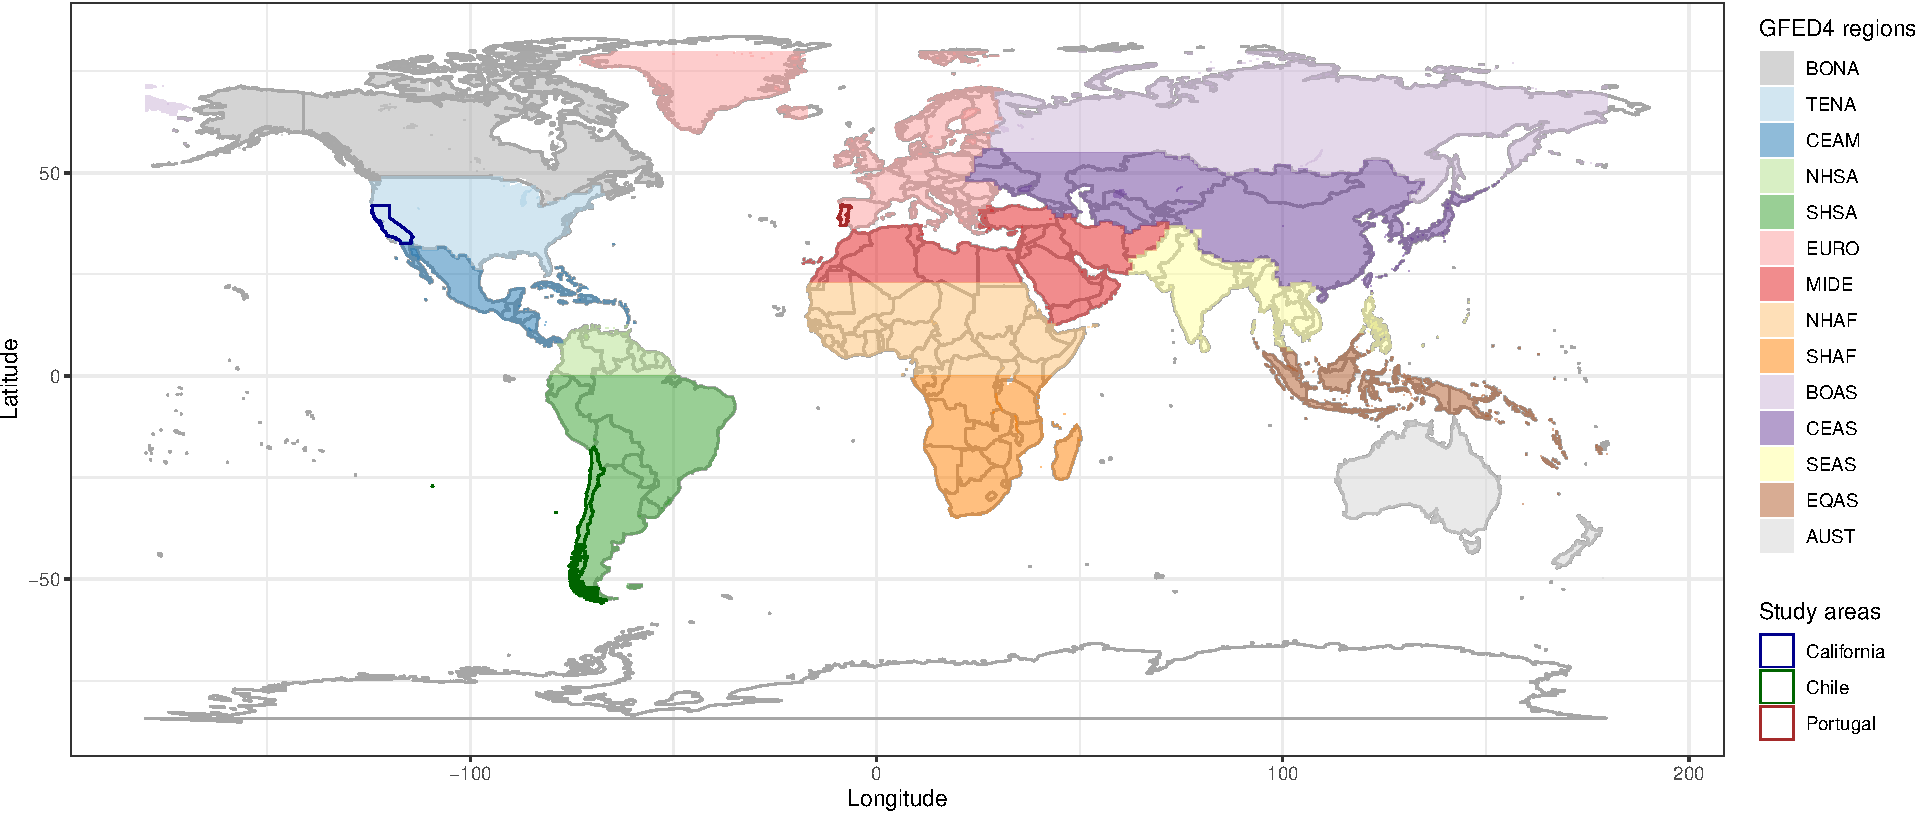
\includegraphics[width=1\linewidth]{article_files/figure-latex/Figure1-1} \caption{\label{fig:Figure1}GFED4 regional classification and the 3 countries selected to showcase the fire forecast performances (California, Chile, and Portugal).}\label{fig:Figure1}
\end{figure}

\begin{verbatim}
## Warning: Removed 104425 rows containing non-finite values (stat_boxplot).
\end{verbatim}

\begin{figure}
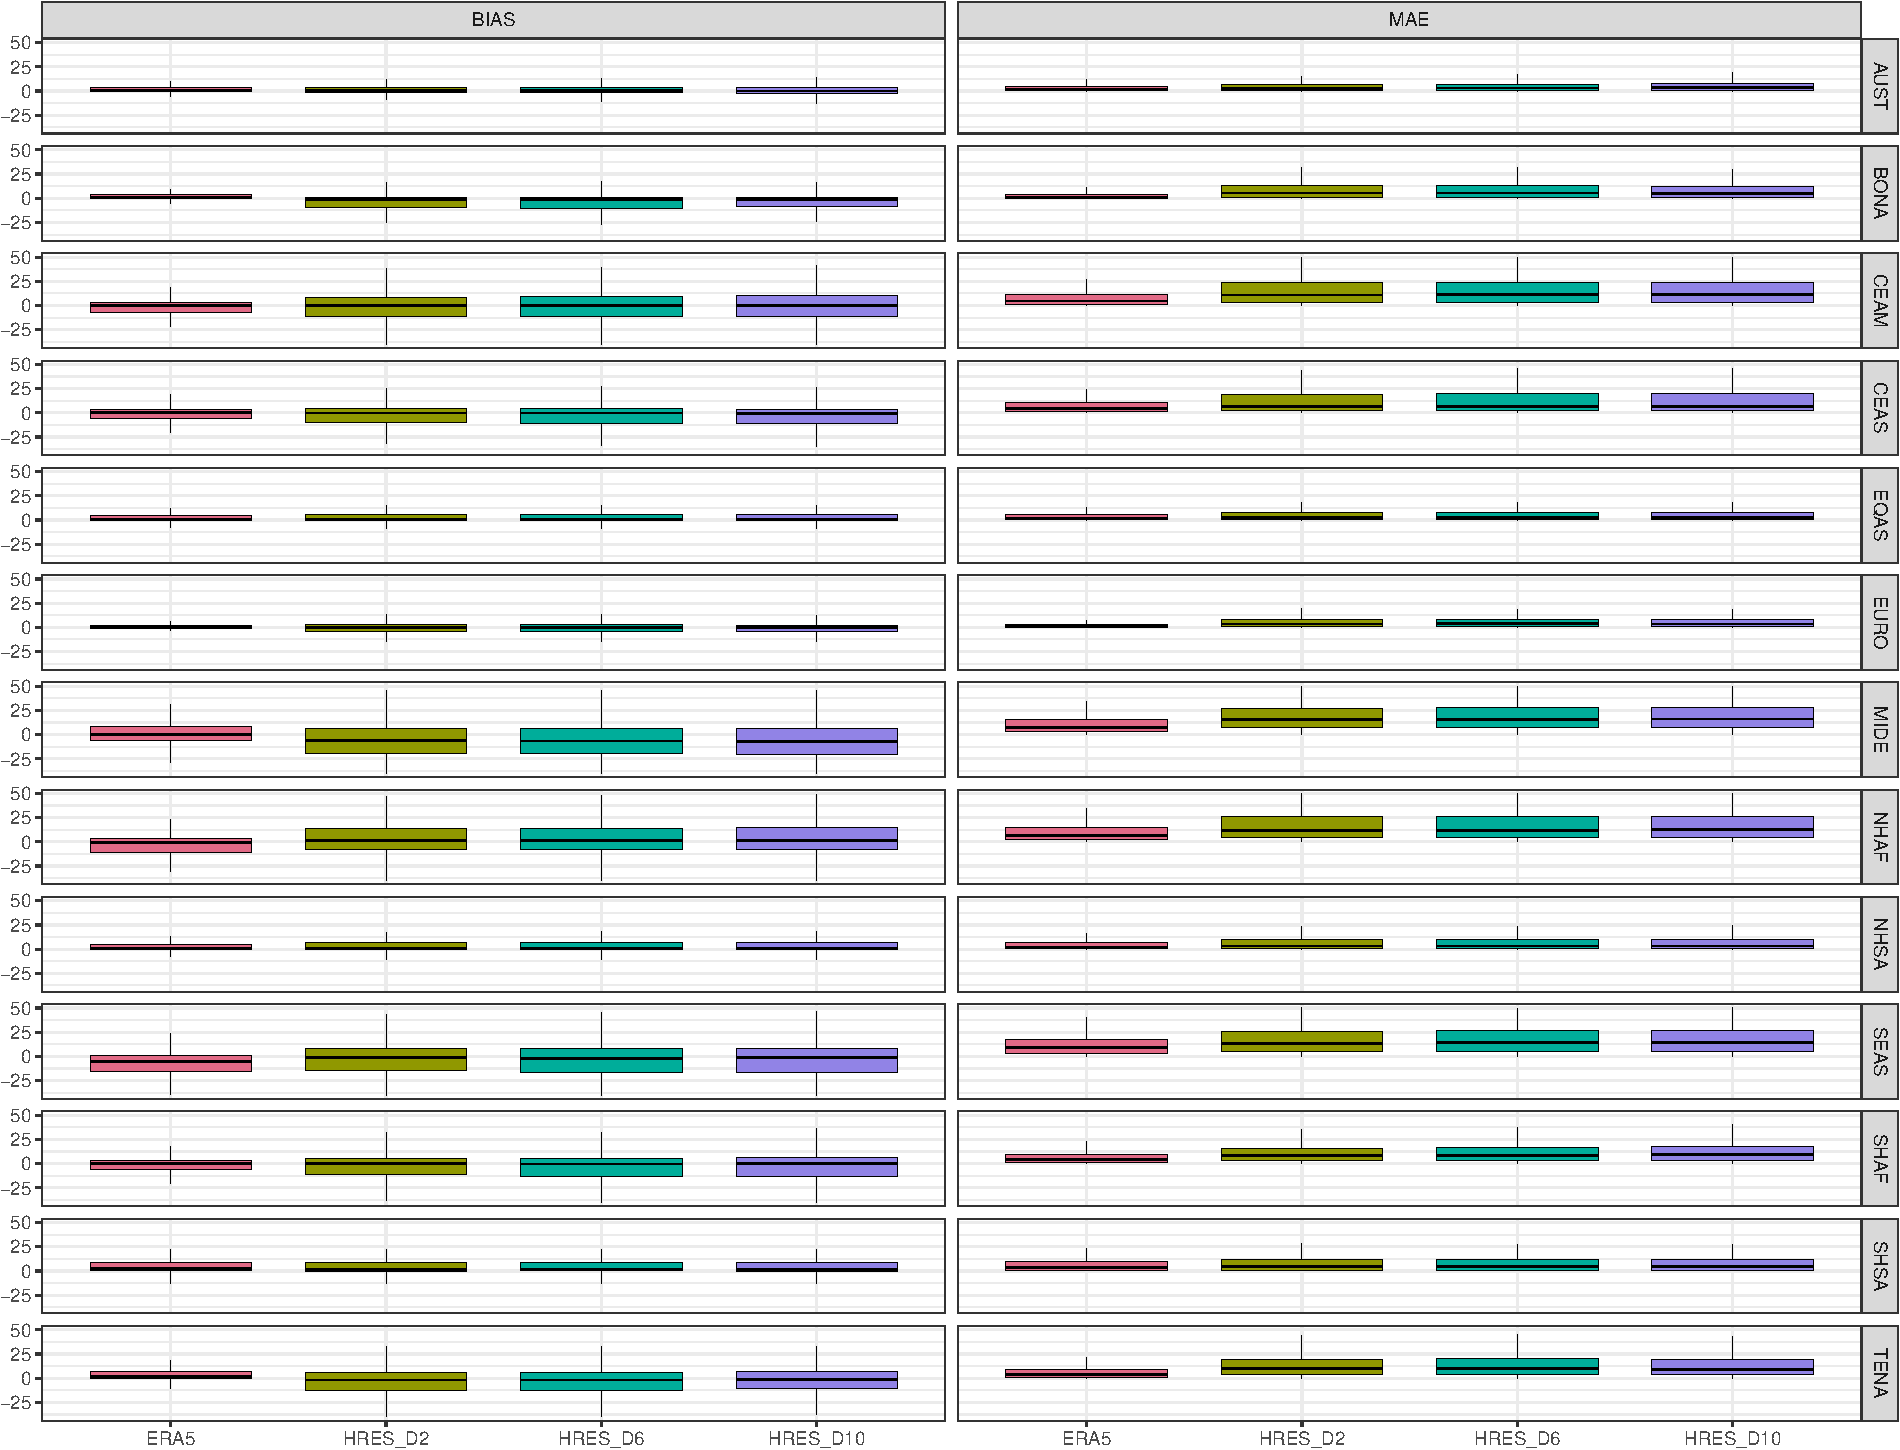
\includegraphics[width=1\linewidth]{article_files/figure-latex/Figure2-1} \caption{\label{fig:Figure3}Comparison between modelled FWI and observed FWI value. FWI are calculated from using ECMWF reanalysis (ERA5) and forecasts at different lead times. The box plots are used to describe the distribution of values accross the observation points for the 2017 Mean Bias (left panel) and the 2017 mean absolute error (right panel).}\label{fig:Figure2}
\end{figure}

Despite its importance the analysis performed using the synop network is
still pointwise and does not cover all the regions where fires are
relevant. Moreover mean biases and MAE are based on the high resolution
forecast. These skill metrics do not provide information about the
performance of the ensemble forecasting as a whole.

\begin{figure}
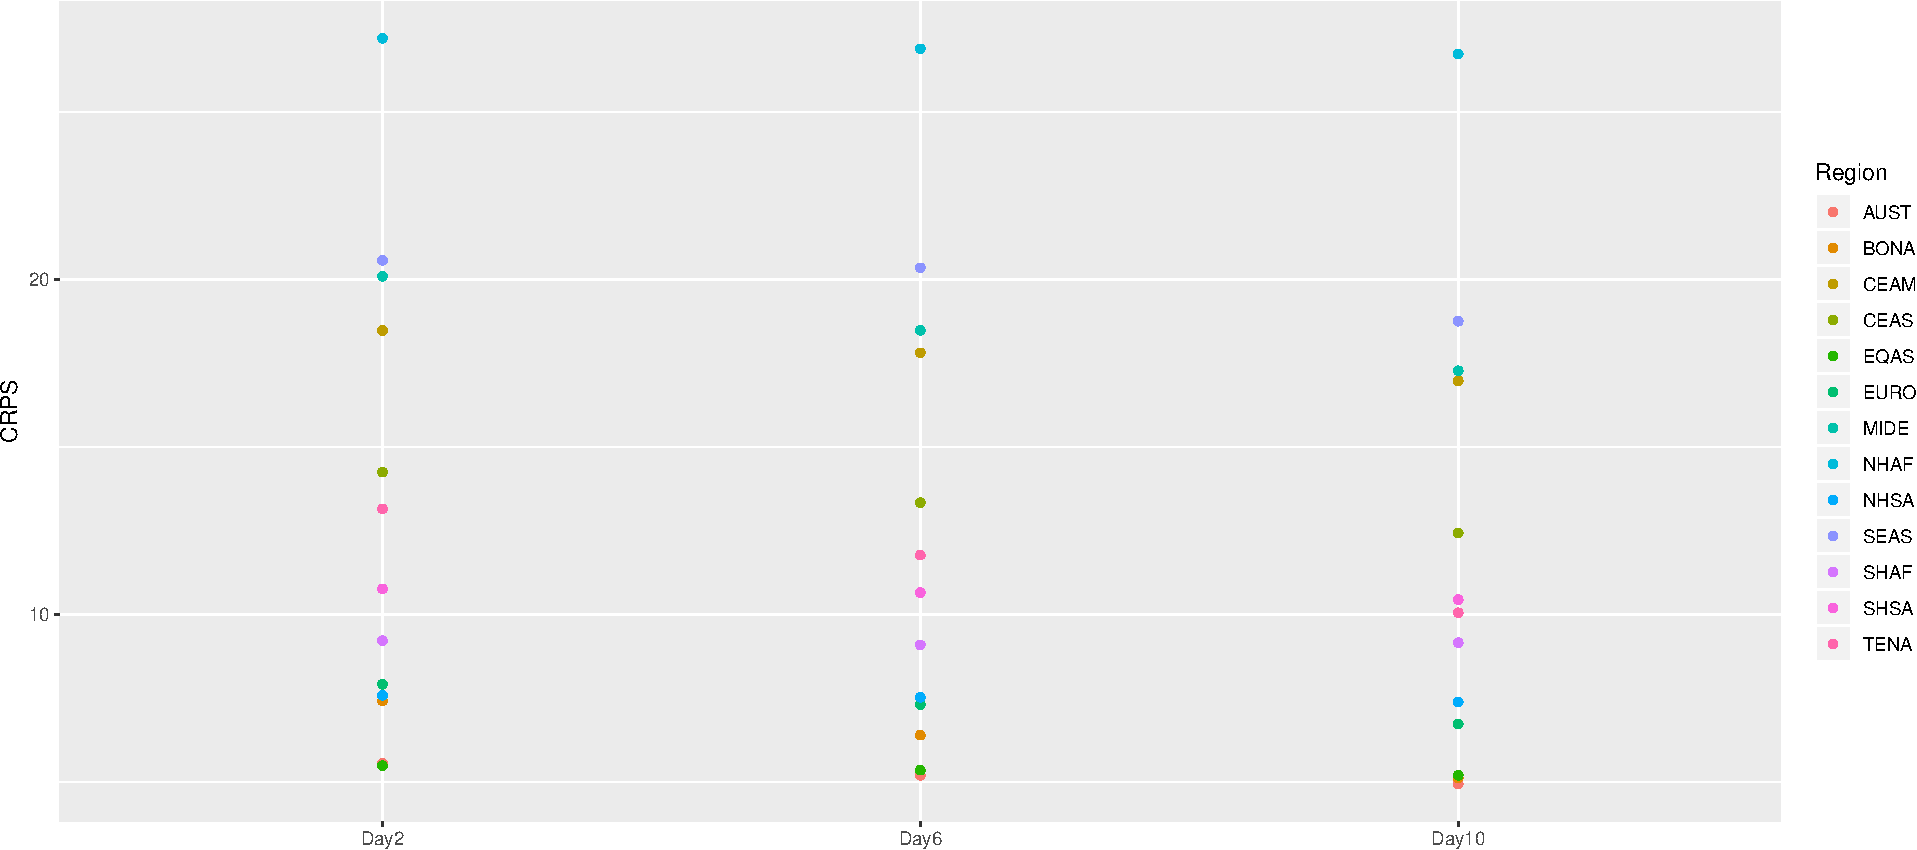
\includegraphics[width=1\linewidth]{article_files/figure-latex/Figure4-1} \caption{\label{fig:Figure4}PUT here crps skills scores.}\label{fig:Figure4}
\end{figure}

\subsection{Skill in detecting fire events}

Conventionally, we assume that an active fire is correctly predicted if
the FWI is greater than the 95\(^{th}\) percentile of its distribution
of values here defined using the ERA5 database.
Figure\textasciitilde{}\ref{fig:pod} shows the mean POD for all events
in 2017 at forecast day 2, 6 and day 10.
Figure\textasciitilde{}\ref{fig:pod} also shows the POD that could be
achieved in the absence of a forecasting system when just using a mean
climatological FWI estimation. Given the intrinsic limitations of the
POD as skill metric, CLIM provides an useful benchmark to understand the
incremental skill provided by the forecast.

At day 2, high latitudes are characterized by POD greater than or equal
to 0.5. These are mostly temperate regions where vegetation is dominated
by forests and fuel is abundant and where fire danger is moisture
limited. In these regions the FWI is a good predictor of fire danger
\citep{digiuseppe:16}. It has to be noted that the FWI does not take
into account management measures that could introduce a relevant number
of ``false-alarm''. Central America, the Middle East and the northern
hemisphere areas, Africa are characterized by a POD in the range 0.3-0.4
as in most of the tropics, where, fires usually occur in grass-shrub
lands. Here fuel is scarce and weather plays a less relevant controlling
role. Also it has to be noted that the statistics here are likely to be
contaminated by many agricultural and prescribed fires that are
considered ``events'' and which would dilute some of the skill in
regions where annual cropland is high or are heavily managed. The
spatial distribution of POD at day 6 is very similar to the
corresponding figures at day 2, just slightly shifted towards lower
values.

One important exception is the extremely good performance of the fire
forecast in Equatorial Asia where the system seems to have a
predictability of 0.9 even at day 6. Also \citet{degroot:07} highlighted
how FWI is not a good indicator in this area and a fire early warning
system should mostly rely on the drought code. Still, there are factors
that could contribute to this enhanced predictability. First fires in
this region are mainly caused by humans for the purposes of cleaning the
land for establishing plantations \citep{field:09,benedetti:16}.
Therefore they occur every season as soon as fuel conditions are
favorable and the ignition is less of a stochastic component. This also
means that the POD statistics are built on a much higher number of
events. Moreover, the strength and prevalence of these fires are
strongly influenced by large-scale climate patterns like El
Ni\{\textasciitilde{}n\}o \cite{field:04} which have been proven being
highly predictable \citep{zhu:15}. The other relevant fact is the almost
null skill globally when a climatological FWI is used highlighting the
added benefit of a forecasting system

\begin{verbatim}
\begin{figure}[htb]
\centering
\includegraphics[width=0.5\textwidth]{POD2.png}\\[0.5cm]
\includegraphics[width=0.5\textwidth]{POD6.png}\\[0.5cm]
\includegraphics[width=0.5\textwidth]{POD10.png}\\[0.5cm]
\includegraphics[width=0.5\textwidth]{PODclima.png}\\[0.5cm]
\caption{Global area averaged Probability of Detection (POD) for  day 2, day 6 and day 10 forecasts and the CLIM run. Pixels where FRP $ \ge $ 0.5 Wm$^{-2}$  are categorized as "yes" events and compared to FWI prediction above the very-high warning level. The global statistic is constructed using all FRP observations detected in 2017 and averaged over the specified regions.} \label{fig:pod}
\end{figure}
\end{verbatim}

\subsection{2017 case studies}

Figure \ref{fig:pod} provides an averaged assessment of the global
performances of the forecasted FWI as a generic indicator of fire
danger. There are regional and seasonal variations to this skill. Also
it is important to understand how the information provided could be used
in real cases when the forecast is intended to aid emergency responses.
Here we will analyses three cases of fire events that took place in
2017, which proved to be an extreme year for fire all across the globe.

The year 2017 started with an extended fire in central Chile that lasted
almost all of January. Strong winds, high temperatures and long-term
drought conditions led to an event that has been described as the worst
wildfire in Chilean history \citep{bowman:18}. Fires in the central
regions of O'Higgins, Maule and B'io B'io south of Santiago were
difficult to control. Although fire activities where recorded since July
2016 they became particularly intense in January 2017. In June, between
17 and 18, another devastating fire hit Portugal. It claimed more than
60 lives mostly recorded in the Pedr'og\textasciitilde{}ao Grande area,
50 km southeast of Coimbra. A persistent heatwave had been building in
the region, with temperatures above 40C, which are highly unusual for
the season. Moreover, relative humidity levels below 30\% had a role to
the intensification of the deflagration and the spread of the wildfire,
which raged out of control for several days \citep{boer:17}. Finally in
Octoberextensive wildfires raced just north of the San Francisco Bay
Area in California causing historic levels of death and destruction.
These named ``Wine Country'' wildfires were the most destructive in
California history, with 44 deaths; the loss of 9,000 buildings; damage
to approximately 21,000 structures; \$10 billion of insured losses; and
substantially greater total economic loss \citep{nauslar:18,mass:19}.

For each case study, the affected area is identified as the minimum area
including all detected active fires (cells with \(FRP > 0.5 Wm^{-2}\))
during the selected time window. Figure \ref{fig:plotthatrulesthemall}
shows the information that could have been provided for the study areas
by the 10-day fire danger high resolution forecasts (HRES), had these
been already available. Each plot shows on the x-axis the dates in which
FRP was observed and, on the y-axis, the dates forecasts were issued.
The cell in the bottom left corner shows the percentage of pixels in the
study area that are expected to be above the 95\(^{th}\) percentile of
the FWI climatology for that pixel. The forecasts for day 2 to day 10
are on the same row. The forecasts issued on the following day are one
row above and so forth. The dashed lines shows the observed fire
radiative power (see also secondary y-axis).

The reader is reminded that active fires are triggered by highly
unpredictable events (ignition) which are not accounted for in the FWI
system. The FWI is not supposed to provide the exact localization of the
event but an indication of potential fire activity. Large areas can be
affected by anomalous conditions in the proximity of where the event
really occurred. However it is noticeable the capability of the forecast
to detect the increase in fire danger associated to the three events.
For the Chile case, for example from mid-January between 70 and 80\% of
the area exceeded the high danger threshold. The FRP spike (occurred on
26th January) highlighting that most of the region was classified at
very high danger almost 10 days ahead. Similarly, the Portugal fire
could have been predicted ten days before, but the California event only
two to three days.

\begin{table*}
\caption{Events summary table.}
\label{tab:fires}
\begin{center}
\begin{tabular}{|llllll|}
\hline
Country  & Region          & Start date & End date &Main event & Location  \\\hline
Chile    & O'Higgins, Maule, B\'io B\'io  & 01-01-2017 & 31-01-2017& 26-01-2017& 36$^\circ$ 46'S; 73$^\circ$ 03'W \\
Portugal & Pedrogao Grande & 01-06-2017 & 30-06-2017 &18-06-2017 & 39$^\circ$ 55'N ; 8$^\circ$ 08' W\\
USA      & California      & 21-09-2017 & 20-10-2017 &09-10-2017& 38$^\circ$ 34'N; 122$^\circ$ 34' W\\
\hline
\end{tabular}
\end{center}
\end{table*}

\begin{verbatim}
\begin{figure}
    \centering
    \begin{subfigure}[b]{0.45\textwidth}
        \centering
        \includegraphics[width=\textwidth]{Chile_boxy_map}
        \caption{Chile}
    \end{subfigure}
    \begin{subfigure}[b]{0.45\textwidth}
        \centering
        \includegraphics[width=\textwidth]{Portugal_boxy_map}
        \caption{Portugal}
    \end{subfigure}
    \begin{subfigure}[b]{0.45\textwidth}
        \centering
        \includegraphics[width=\textwidth]{California_boxy_map}
        \caption{California}
    \end{subfigure}
    \caption{Comparison of Fire Radiative Power (gray dashed line with axis on the right hand side) with FWI forecasted using the deterministic high resolution model for California, Portugal and  Chile. FWI is color coded based on the percentage of pixels exceeding the high danger level calculated at the country/state level. Each of the panel refers to a specific fire event described in the text and the statistics have been calculated over the red boxes.} \label{fig:plotthatrulesthemall}
\end{figure}
\end{verbatim}

One of the advantages of developing a probabilistic ensemble prediction
system (ENS) for fire danger is the possibility to assess the confidence
in the model forecast, at least from the point of view of the
uncertainties in weather forcings. Admittedly, the use of this type of
information is not straightforward as many studies have highlighted
\citep{pappenberger:13,palmer:00}. This difficulty steams from the fact
that in many response systems an activation is conditional to the
excedance of deterministic threshold. Instead, in a probabilistic
approach what is provided is the \{\it probability\} of exceedance a
certain values and this is often perceived as a degradation of the
information values \citep{richardson:00}. However by using the
probabilistic component of the system, it is possible to understand how
consistent the fire danger forecast is with respect to slightly
different forecast scenarios. To highlight the information that can be
added with the use of the ensemble prediction system, Figure
\ref{fig:fire_ensfwi} shows the progression of 10-day forecasts for the
major fire events (corresponding to the peak of observed FRP in figure
\ref{fig:plotthatrulesthemall}) in the three case studies. In this case
we concentrate on a specific location (model grid box) whose coordinates
are specified in table \ref{tab:fires}. In this plot, there is very high
consistency between HRES and ENS, with the former falling generally
close to the ensemble median. In addition, the bulk of ensemble members
falls in the yellow region which identifies very high danger. It is this
consistency and persistence of very high danger over time that could
have helped users gain confidence in the forecast, had that been already
available. While these events were all considered catastrophic in terms
of impacts, it is noticeable that, at all forecast ranges, fire danger
would have been classified as very-high but not extreme by the exclusive
use of the high resolution forecast. However in all three cases by
looking at the full distribution of FWI values provided by the ensemble,
it is clear that some of the forecasts were hinting at the possibility
for extreme conditions.

Thus is there an enhanced accuracy in the forecast produced with the use
of the ensemble forecasting system? Figure \ref{fig:fire_enspod} shows
the probability of detection calculated over the three fire regions (see
red box in Figure \ref{fig:plotthatrulesthemall} for the geographical
extents of these areas) using all the ensemble members. The high
resolution forecast (red dots) is not in all cases the most skillful
prediction despite the increased resolution. It is interesting to notice
how in the California case, for example, many of the ensemble members
perform consistently better than the high resolution run up to 6 days
ahead.

\begin{verbatim}
\begin{figure}
    \centering
    \begin{subfigure}[b]{0.45\textwidth}
        \centering
        \includegraphics[width=\textwidth]{Chile_ENSfwi}
        \caption{Chile}
    \end{subfigure}
    \begin{subfigure}[b]{0.45\textwidth}
        \centering
        \includegraphics[width=\textwidth]{Portugal_ENSfwi}
        \caption{Portugal}
    \end{subfigure}
    \begin{subfigure}[b]{0.45\textwidth}
        \centering
        \includegraphics[width=\textwidth]{California_ENSfwi}
        \caption{California}
    \end{subfigure}
    \caption{Fire Weather Index distribution at the location and date specified as "main event" in table \ref{tab:fires}. The sequence of box plots refer to different forecast days. The warning levels are calculated using the methodology explained in section 3. The high resolution prediction is represented with a red dot. In the box plot horizontal lines identify the median and the 25\% and 75\% percentile. The height of the box identify the inter-quartile range. The upper and lower whiskers represent the interval up to $\pm$ 1.5 times the middle quartile interval and black dots are used for the outliers.} \label{fig:fire_ensfwi}
\end{figure}

\begin{figure}
    \centering
    \begin{subfigure}[b]{0.45\textwidth}
        \centering
        \includegraphics[width=\textwidth]{Chile_ENS}
        \caption{Chile}
    \end{subfigure}
    \begin{subfigure}[b]{0.45\textwidth}
        \centering
        \includegraphics[width=\textwidth]{Portugal_ENS}
        \caption{Portugal}
    \end{subfigure}
    \begin{subfigure}[b]{0.45\textwidth}
        \centering
        \includegraphics[width=\textwidth]{California_ENS}
        \caption{California}
    \end{subfigure}
    \caption{Probability of detection (POD) as a function of forecast horizon for the ensemble prediction system. The POD is constructed matching active fires with FWI in the very-high danger class in the three selected case study areas. The POD for the high resolution run is shown with red dots. In the box plot horizontal lines identify the median and the 25\% and 75\% percentile. The length of the box identify the middle quartile interval. The upper and lower whiskers represent the interval up to $\pm$ 1.5 times the middle quartile interval and black dots are used for the outliers.} \label{fig:fire_enspod}
\end{figure}
\end{verbatim}

\conclusions

In the last years, ECMWF has been involved in the EFFIS development by
providing weather forcing and fire danger calculations using its
medium-range weather forecasts. Global fields of FWI are calculated
daily using the high-resolution (9 km) forecast up to 10 days ahead. The
18 km resolution ensemble prediction system provides additional 51
realizations based on slightly different initial conditions and/or using
different model configurations \citep{molteni:96}. These datasets are
freely available in line with the data and information policy of the
Copernicus program which intends to provide users with free, full and
open access to environmental data.

Using one year of operational service in 2017 we have showcased the
potential of the use of weather forecasts to support the monitoring of
fire danger conditions and planning in case of a potential emergency. By
applying a model based definition of warning levels to the FWI we have
shown that it provides a probability of detection (POD) for fire
activity that is often above 60\% at day 2. Mid and high latitude
forested areas, where fuel is abundant have the highest predictability
while in savana/shrub-land regions the relationship between FWI and fire
occurrence weakens. With the exception of Equatorial Asia which shows a
POD in the range of 0.9 the average mean POD falls below the 0.6
threshold by day 6 on average highlighting that this might be consider a
rough estimation of the limit for a skillful prediction which could
justify the use of prediction at this stage. However there are regional
and case-specific variations to this limit. Using the three large fire
events of 2017 in Chile, Portugal and California, as examples, we have
shown that accurate forecasts can be achieved up to 10 days ahead.

Another interesting aspect attached to the use of weather forecasts is
the use of probabilistic information. The quantification of forecast
uncertainties through the use of ensemble predictions is something still
pretty new in fire forecasting. However it opens great opportunities in
terms of adding a confidence level to the the fire prediction.


\codeavailability{The code to generate the results of this work is available as vignette
of the caliver R package: Verification of fire danger classes.} %% use this section when having only software code available





%%%%%%%%%%%%%%%%%%%%%%%%%%%%%%%%%%%%%%%%%%
%% optional

%%%%%%%%%%%%%%%%%%%%%%%%%%%%%%%%%%%%%%%%%%

%%%%%%%%%%%%%%%%%%%%%%%%%%%%%%%%%%%%%%%%%%
\authorcontribution{FDG wrote the \ldots{}} %% optional section

%%%%%%%%%%%%%%%%%%%%%%%%%%%%%%%%%%%%%%%%%%
\competinginterests{The authors declare no competing interests.} %% this section is mandatory even if you declare that no competing interests are present

%%%%%%%%%%%%%%%%%%%%%%%%%%%%%%%%%%%%%%%%%%

%%%%%%%%%%%%%%%%%%%%%%%%%%%%%%%%%%%%%%%%%%
\begin{acknowledgements}
This work was founded by the EU Project ANYWHERE (Contract 700099) and
the Global Fire Contract 389730 between the Joint Research Centre and
ECMWF.
\end{acknowledgements}

%% REFERENCES
%% DN: pre-configured to BibTeX for rticles

%% The reference list is compiled as follows:
%%
%% \begin{thebibliography}{}
%%
%% \bibitem[AUTHOR(YEAR)]{LABEL1}
%% REFERENCE 1
%%
%% \bibitem[AUTHOR(YEAR)]{LABEL2}
%% REFERENCE 2
%%
%% \end{thebibliography}

%% Since the Copernicus LaTeX package includes the BibTeX style file copernicus.bst,
%% authors experienced with BibTeX only have to include the following two lines:
%%
\bibliographystyle{copernicus}
\bibliography{references.bib}
%%
%% URLs and DOIs can be entered in your BibTeX file as:
%%
%% URL = {http://www.xyz.org/~jones/idx_g.htm}
%% DOI = {10.5194/xyz}


%% LITERATURE CITATIONS
%%
%% command                        & example result
%% \citet{jones90}|               & Jones et al. (1990)
%% \citep{jones90}|               & (Jones et al., 1990)
%% \citep{jones90,jones93}|       & (Jones et al., 1990, 1993)
%% \citep[p.~32]{jones90}|        & (Jones et al., 1990, p.~32)
%% \citep[e.g.,][]{jones90}|      & (e.g., Jones et al., 1990)
%% \citep[e.g.,][p.~32]{jones90}| & (e.g., Jones et al., 1990, p.~32)
%% \citeauthor{jones90}|          & Jones et al.
%% \citeyear{jones90}|            & 1990

\end{document}
